\documentclass[12pt]{article}
\usepackage{amsmath,amssymb,amsfonts}
\usepackage{tikz}
\usepackage{float}
\usepackage[margin=0.5in]{geometry}
\newcommand{\pdata}{p_\mathrm{data}}
\begin{document}
\begin{center}
Name: \rule{3in}{0.4pt} \hfill Total: 18 points
\end{center}

As usual, let $p_\mathrm{data}$ be the unknown target distribution, and $x^{(i)} \in \mathbb{R}^d$ be iid samples according to $p_\mathrm{data}$ that are given to us.
Let $X_1 \sim p_\mathrm{data}$ and $X_0 \sim \mu$, where $\mu$ is an easy-to-sample distribution, e.g., a standard normal distribution in $\mathbb{R}^d$.
In flow matching, the goal is to learn a vector field, $v_t(x),$ such that its flow $\varphi^t(x)$ satisfies
$$\varphi^1_\sharp \mu = p_\mathrm{data}.$$

To do this, we consider the intermediate marginal densities, $\rho_t,$ which satisfy the continuity equation, as a total expectation:
\begin{equation}
	\rho_t(x) = \mathbb{E}_{z \sim q_Z} p_{X_t|Z}(x|z),
\end{equation}
where $Z = (X_0, X_1)$ is chosen according to a joint distribution $q_Z.$ Here, $p_{X_t|Z}$ is the conditional density of $X_t$.    

\begin{enumerate}
	\item Let $p_{X_t|Z}= \mathcal{N}(m_t, \sigma_t^2\: \mathrm{Id}),$ with $m_t((x_0, x_1)) = tx_1 + (1-t)x_0.$ Then, the path connecting $X_0$ and $X_1$ where $(X_0, X_1) \sim q_Z,$ becomes a straight line for any choice of coupling $q_Z.$ True or False? Justify your answer. (2 points)
	\vfill
	\item True or false: the OT-CFM flow $\varphi^1$ is the same as the Brenier transport map (2 points) 
	\vfill

	
	\item Match the learned vector fields from three different conditional flow matching algorithms: CFM, OT-CFM and stochastic interpolants. 
	In stochastic interpolants, $q_Z = \rho_0(x_0)\:\rho_1(x_1)$ and $m_t((x_0, x_1)) = \cos(\pi t/2)x_0 + \sin(\pi t/2)x_1.$  
	The distribution $\pdata$ is the following 2 moons distribution:
	\begin{figure}[H]
		\centering
		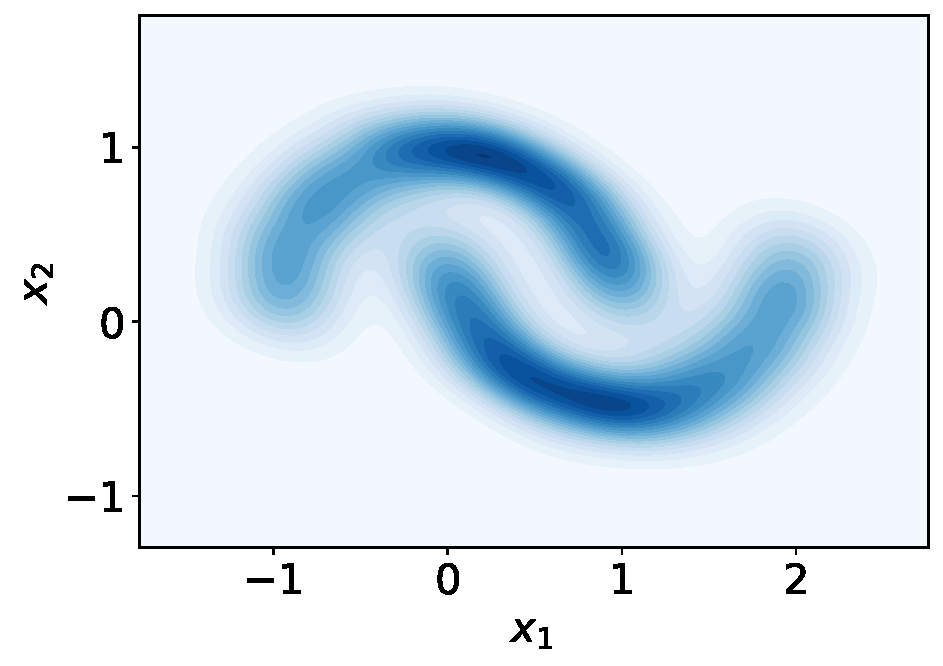
\includegraphics[width=0.3\textwidth]{two_moons_kde.pdf}
		\caption{$\pdata$}
	\end{figure}
	\begin{figure}[H]
		\centering
		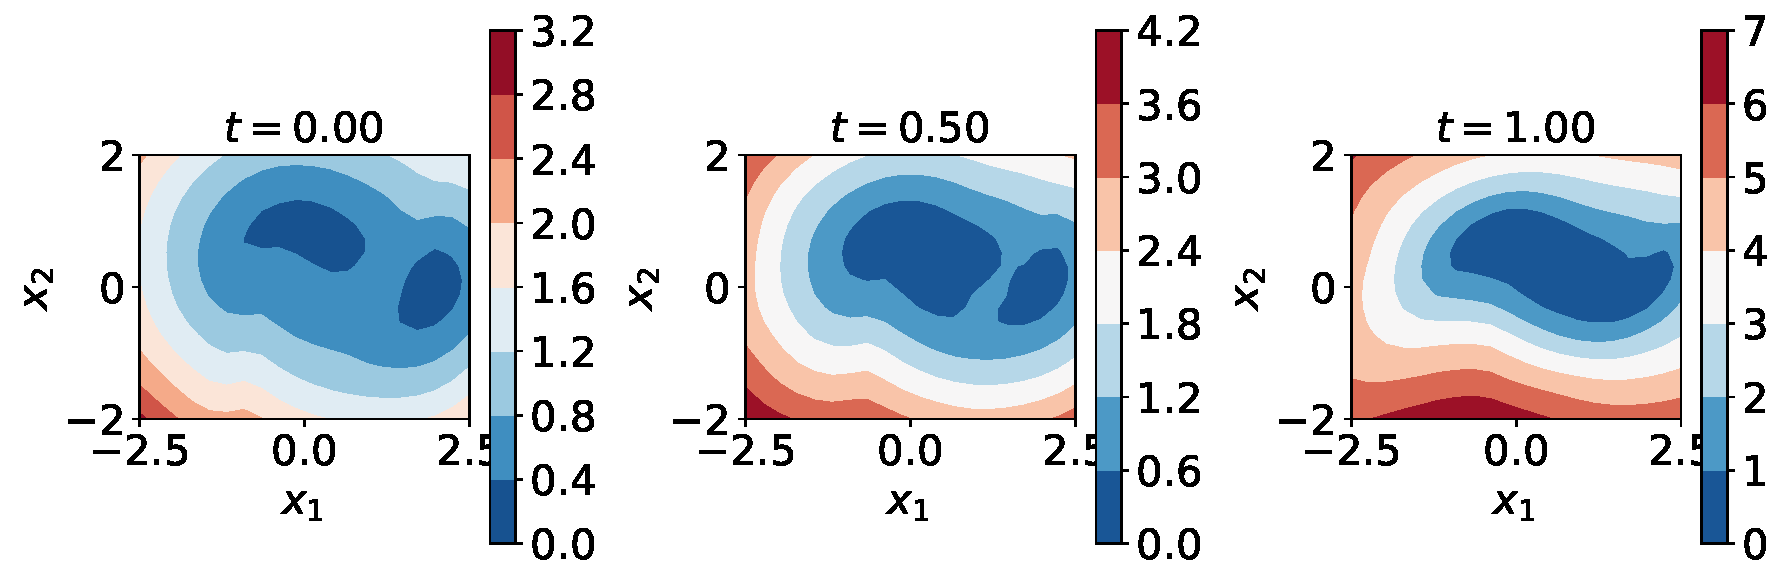
\includegraphics[width=0.6\textwidth]{otcfm_vector_field.pdf} \\
		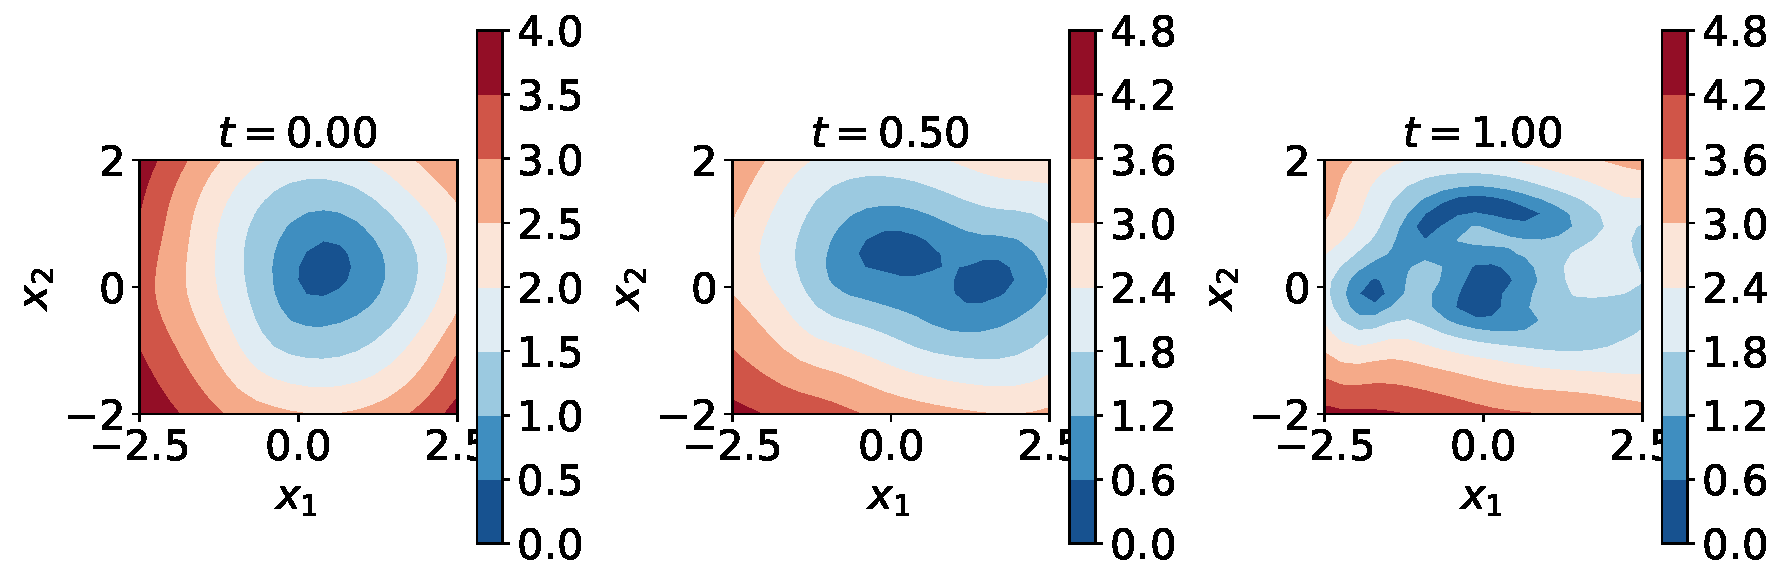
\includegraphics[width=0.6\textwidth]{cfm_vector_field.pdf} \\
		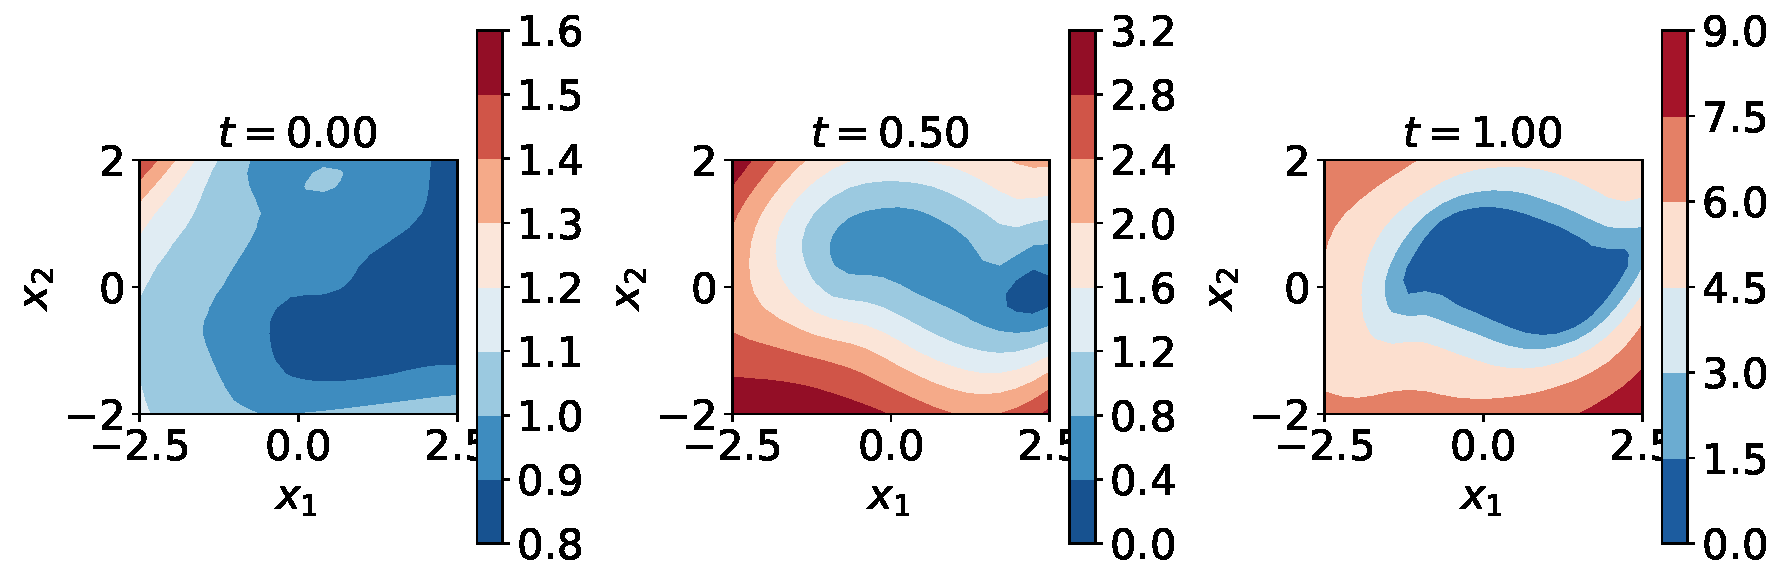
\includegraphics[width=0.6\textwidth]{si_otcfm_vector_field.pdf}
		\caption{Row 1: ........, Row 2: ........, Row 3:..........}
	\end{figure}
	3 points for the correct match, 3 for the correct reasoning.
	\vfill
	



	\item Match the learned paths below. The starting point, $x_0$, is marked as a square and the end point, $x_1,$ is marked as a circle. Justify your answer (5 points)
	\begin{figure}[H]
		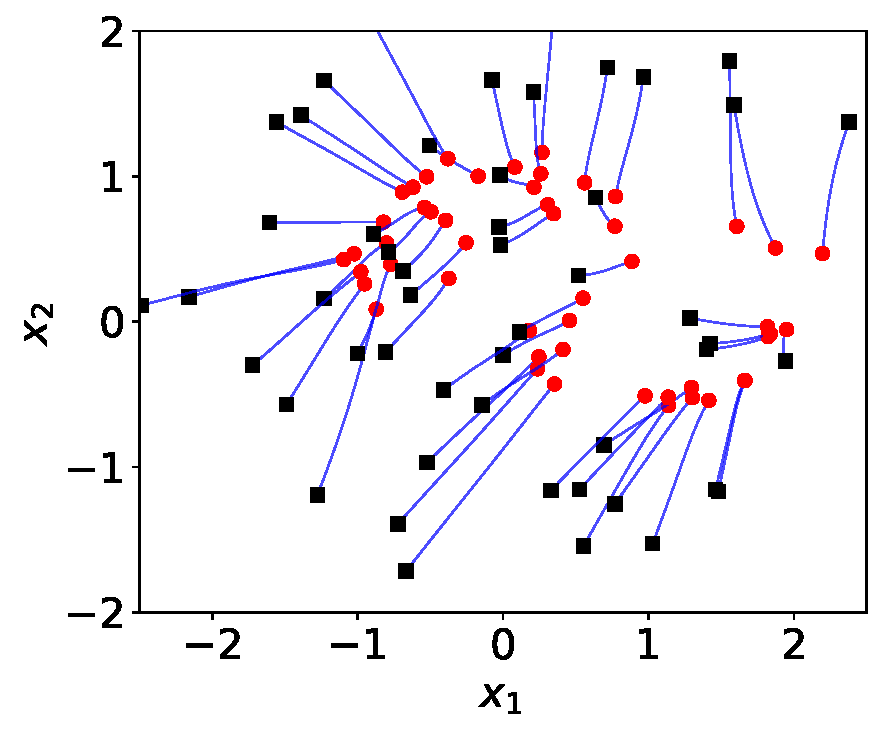
\includegraphics[width=0.3\textwidth]{otcfm_trajectories.pdf}
		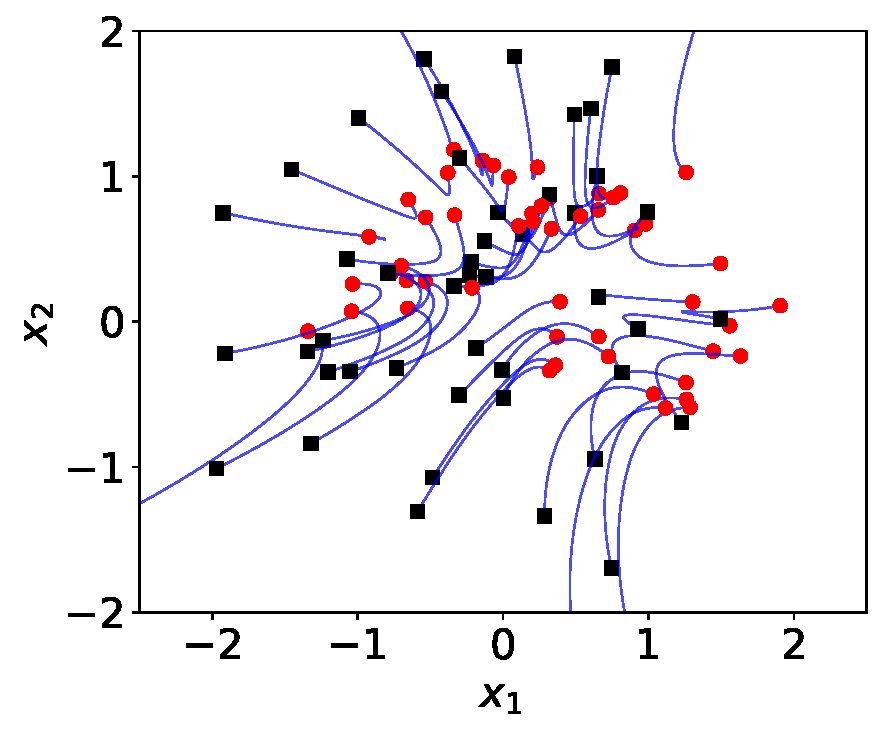
\includegraphics[width=0.3\textwidth]{cfm_trajectories.pdf}
		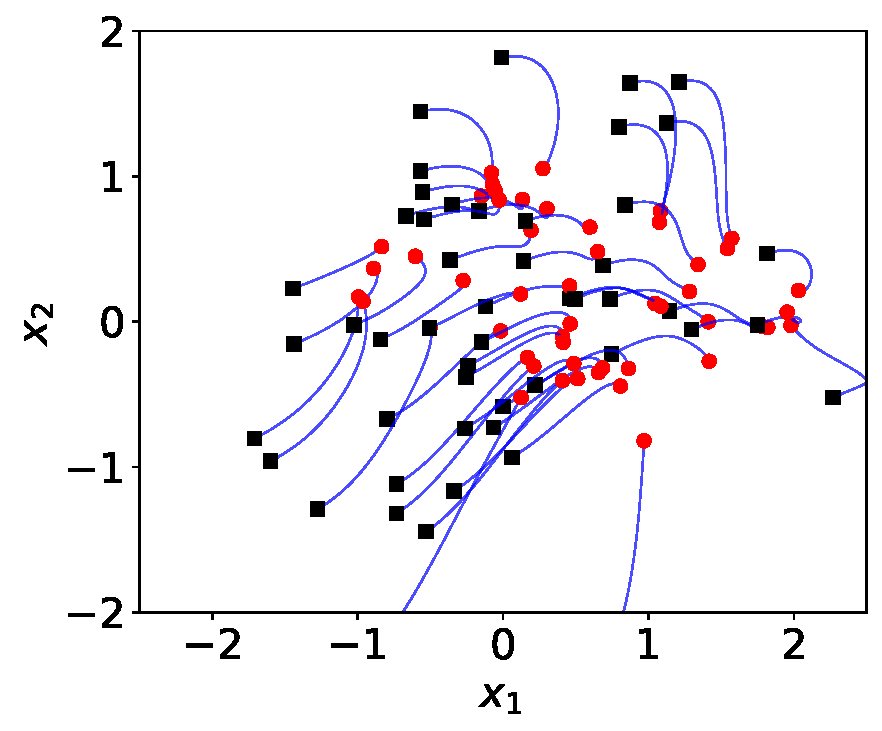
\includegraphics[width=0.3\textwidth]{si_otcfm_trajectories.pdf}
		\caption{Left:......., Center:.............., Right:..........}
	\end{figure}
	\vfill


	


	\item Now consider a new process: $X_0 = \alpha_t X_1 + \sigma_t \epsilon,$ where $\epsilon \sim \mathcal{N}(0, \mathrm{Id}).$ This is a noising process in a diffusion model. 
	What is the conditional expectation of $p_\mathrm{data}$ given a noised sample, $X_0$? (1 point) If $\alpha_t$ decreases with $t$ and $\sigma_t$ increases with $t,$ when is the conditional expectation a good approximation of a sample $X_1 \sim \pdata$, for small or large $t$?
	Explain (2 points) 
	\vfill


\end{enumerate}


\end{document}
